% Options for packages loaded elsewhere
\PassOptionsToPackage{unicode}{hyperref}
\PassOptionsToPackage{hyphens}{url}
\PassOptionsToPackage{dvipsnames,svgnames,x11names}{xcolor}
%
\documentclass[
  letterpaper,
  DIV=11,
  numbers=noendperiod]{scrartcl}

\usepackage{amsmath,amssymb}
\usepackage{iftex}
\ifPDFTeX
  \usepackage[T1]{fontenc}
  \usepackage[utf8]{inputenc}
  \usepackage{textcomp} % provide euro and other symbols
\else % if luatex or xetex
  \usepackage{unicode-math}
  \defaultfontfeatures{Scale=MatchLowercase}
  \defaultfontfeatures[\rmfamily]{Ligatures=TeX,Scale=1}
\fi
\usepackage{lmodern}
\ifPDFTeX\else  
    % xetex/luatex font selection
\fi
% Use upquote if available, for straight quotes in verbatim environments
\IfFileExists{upquote.sty}{\usepackage{upquote}}{}
\IfFileExists{microtype.sty}{% use microtype if available
  \usepackage[]{microtype}
  \UseMicrotypeSet[protrusion]{basicmath} % disable protrusion for tt fonts
}{}
\makeatletter
\@ifundefined{KOMAClassName}{% if non-KOMA class
  \IfFileExists{parskip.sty}{%
    \usepackage{parskip}
  }{% else
    \setlength{\parindent}{0pt}
    \setlength{\parskip}{6pt plus 2pt minus 1pt}}
}{% if KOMA class
  \KOMAoptions{parskip=half}}
\makeatother
\usepackage{xcolor}
\setlength{\emergencystretch}{3em} % prevent overfull lines
\setcounter{secnumdepth}{-\maxdimen} % remove section numbering
% Make \paragraph and \subparagraph free-standing
\makeatletter
\ifx\paragraph\undefined\else
  \let\oldparagraph\paragraph
  \renewcommand{\paragraph}{
    \@ifstar
      \xxxParagraphStar
      \xxxParagraphNoStar
  }
  \newcommand{\xxxParagraphStar}[1]{\oldparagraph*{#1}\mbox{}}
  \newcommand{\xxxParagraphNoStar}[1]{\oldparagraph{#1}\mbox{}}
\fi
\ifx\subparagraph\undefined\else
  \let\oldsubparagraph\subparagraph
  \renewcommand{\subparagraph}{
    \@ifstar
      \xxxSubParagraphStar
      \xxxSubParagraphNoStar
  }
  \newcommand{\xxxSubParagraphStar}[1]{\oldsubparagraph*{#1}\mbox{}}
  \newcommand{\xxxSubParagraphNoStar}[1]{\oldsubparagraph{#1}\mbox{}}
\fi
\makeatother


\providecommand{\tightlist}{%
  \setlength{\itemsep}{0pt}\setlength{\parskip}{0pt}}\usepackage{longtable,booktabs,array}
\usepackage{calc} % for calculating minipage widths
% Correct order of tables after \paragraph or \subparagraph
\usepackage{etoolbox}
\makeatletter
\patchcmd\longtable{\par}{\if@noskipsec\mbox{}\fi\par}{}{}
\makeatother
% Allow footnotes in longtable head/foot
\IfFileExists{footnotehyper.sty}{\usepackage{footnotehyper}}{\usepackage{footnote}}
\makesavenoteenv{longtable}
\usepackage{graphicx}
\makeatletter
\def\maxwidth{\ifdim\Gin@nat@width>\linewidth\linewidth\else\Gin@nat@width\fi}
\def\maxheight{\ifdim\Gin@nat@height>\textheight\textheight\else\Gin@nat@height\fi}
\makeatother
% Scale images if necessary, so that they will not overflow the page
% margins by default, and it is still possible to overwrite the defaults
% using explicit options in \includegraphics[width, height, ...]{}
\setkeys{Gin}{width=\maxwidth,height=\maxheight,keepaspectratio}
% Set default figure placement to htbp
\makeatletter
\def\fps@figure{htbp}
\makeatother

\KOMAoption{captions}{tableheading}
\makeatletter
\@ifpackageloaded{caption}{}{\usepackage{caption}}
\AtBeginDocument{%
\ifdefined\contentsname
  \renewcommand*\contentsname{Table of contents}
\else
  \newcommand\contentsname{Table of contents}
\fi
\ifdefined\listfigurename
  \renewcommand*\listfigurename{List of Figures}
\else
  \newcommand\listfigurename{List of Figures}
\fi
\ifdefined\listtablename
  \renewcommand*\listtablename{List of Tables}
\else
  \newcommand\listtablename{List of Tables}
\fi
\ifdefined\figurename
  \renewcommand*\figurename{Figure}
\else
  \newcommand\figurename{Figure}
\fi
\ifdefined\tablename
  \renewcommand*\tablename{Table}
\else
  \newcommand\tablename{Table}
\fi
}
\@ifpackageloaded{float}{}{\usepackage{float}}
\floatstyle{ruled}
\@ifundefined{c@chapter}{\newfloat{codelisting}{h}{lop}}{\newfloat{codelisting}{h}{lop}[chapter]}
\floatname{codelisting}{Listing}
\newcommand*\listoflistings{\listof{codelisting}{List of Listings}}
\makeatother
\makeatletter
\makeatother
\makeatletter
\@ifpackageloaded{caption}{}{\usepackage{caption}}
\@ifpackageloaded{subcaption}{}{\usepackage{subcaption}}
\makeatother

\ifLuaTeX
  \usepackage{selnolig}  % disable illegal ligatures
\fi
\usepackage{bookmark}

\IfFileExists{xurl.sty}{\usepackage{xurl}}{} % add URL line breaks if available
\urlstyle{same} % disable monospaced font for URLs
\hypersetup{
  pdftitle={Primera Clase de Álgebra Lineal},
  colorlinks=true,
  linkcolor={blue},
  filecolor={Maroon},
  citecolor={Blue},
  urlcolor={Blue},
  pdfcreator={LaTeX via pandoc}}


\title{Primera Clase de Álgebra Lineal}
\author{}
\date{}

\begin{document}
\maketitle


\subsubsection{Aplicaciones de las
Matrices}\label{aplicaciones-de-las-matrices}

\begin{itemize}
\item
  \textbf{Aplicaciones de las Matrices}
\item
  \textbf{Ingeniería}: Usadas para el análisis de estructuras, sistemas
  de control y simulaciones.
\item
  \textbf{Ciencias de la Computación}: Algoritmos gráficos,
  procesamiento de imágenes, y redes neuronales.
\item
  \textbf{Economía}: Modelos de análisis económico, optimización de
  recursos y análisis de riesgos.
\item
  \textbf{Física}: Representación de ecuaciones en dinámica y mecánica
  cuántica.
\end{itemize}

\begin{center}\rule{0.5\linewidth}{0.5pt}\end{center}

\begin{figure}[H]

{\centering 
\includegraphics{figures/figuralineal.jpg}

}

\caption{Aplicaciones de Matrices}

\end{figure}%

\begin{center}\rule{0.5\linewidth}{0.5pt}\end{center}

\subsubsection{Diapositiva 4: Aplicaciones Avanzadas de las
Matrices}\label{diapositiva-4-aplicaciones-avanzadas-de-las-matrices}

\textbf{Aplicaciones Avanzadas de las Matrices}

\begin{itemize}
\tightlist
\item
  \textbf{Redes Sociales}: Utilizadas para el análisis de conexiones
  entre usuarios y recomendaciones de amistades.
\item
  \textbf{Procesamiento de Señales}: Aplicadas en la compresión de audio
  y video, filtrado de señales y reconocimiento de voz.
\item
  \textbf{Aprendizaje Automático}: Matrices son fundamentales en
  algoritmos de aprendizaje automático como la regresión lineal y las
  redes neuronales.
\item
  \textbf{Criptografía}: Matrices se utilizan en algoritmos de cifrado y
  descifrado para garantizar la seguridad de la información.
\end{itemize}

\begin{center}\rule{0.5\linewidth}{0.5pt}\end{center}

\begin{figure}[H]

{\centering 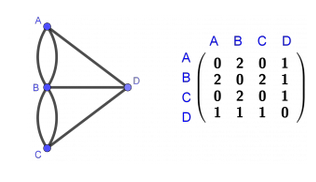
\includegraphics{figures/grafo.png}

}

\caption{Aplicaciones Avanzadas de Matrices}

\end{figure}%

\begin{center}\rule{0.5\linewidth}{0.5pt}\end{center}

\subsubsection{Nomenclatura y Definición de
Matrices}\label{nomenclatura-y-definiciuxf3n-de-matrices}

\textbf{Nomenclatura y Dimensiones de las Matrices}

\begin{itemize}
\tightlist
\item
  \textbf{Matriz}: Un arreglo rectangular de números dispuestos en filas
  y columnas.
\item
  \textbf{Elementos de una matriz}: \(a_{ij}\) representa el elemento en
  la i-ésima fila y j-ésima columna.
\item
  \textbf{Dimensiones de una matriz}: Si una matriz tiene m filas y n
  columnas, se describe como una matriz de \(m \times n\).
\end{itemize}

\begin{center}\rule{0.5\linewidth}{0.5pt}\end{center}

\textbf{Ejemplo de Matriz}: \[ A = \begin{bmatrix}
1 & 2 & 3 \\
4 & 5 & 6
\end{bmatrix} \] Esta es una matriz de \(2    \times 3\).

\begin{center}\rule{0.5\linewidth}{0.5pt}\end{center}

\begin{center}\rule{0.5\linewidth}{0.5pt}\end{center}

\subsubsection{Operaciones con Matrices}\label{operaciones-con-matrices}

\textbf{Operaciones Básicas con Matrices}

\begin{itemize}
\tightlist
\item
  \textbf{Suma de Matrices}: Las matrices se suman elemento por
  elemento.
\end{itemize}

\[\begin{bmatrix} 1 & 3 \\ 1 & 0 \end{bmatrix} + \begin{bmatrix} 0 & 0 \\ 7 & 5 \end{bmatrix} = \begin{bmatrix} 1 & 3 \\ 8 & 5 \end{bmatrix}\]

\begin{center}\rule{0.5\linewidth}{0.5pt}\end{center}

\begin{itemize}
\tightlist
\item
  \textbf{Multiplicación por un Escalar}: Todos los elementos de la
  matriz se multiplican por el escalar.
\end{itemize}

\[3     \times \begin{bmatrix} 1 & 3 \\ 1 & 0 \end{bmatrix} = \begin{bmatrix} 3 & 9 \\ 3 & 0 \end{bmatrix}\]

\begin{center}\rule{0.5\linewidth}{0.5pt}\end{center}

\begin{itemize}
\tightlist
\item
  \textbf{Multiplicación de Matrices}: El elemento en la posición
  \((i, j)\) del producto es el producto punto de la fila i de la
  primera matriz y la columna j de la segunda matriz.
\end{itemize}

\[ \begin{bmatrix} 1 & 2 \\ 3 & 4 \end{bmatrix}     \times \begin{bmatrix} 2 & 0 \\ 1 & 2 \end{bmatrix} = \begin{bmatrix} 4 & 4 \\ 10 & 8 \end{bmatrix}\]

\begin{center}\rule{0.5\linewidth}{0.5pt}\end{center}

La multiplicación de matrices se define como sigue: \[
(C)_{ij} = \sum_{k=1}^n A_{ik} B_{kj}
\] Donde:

\begin{itemize}
\tightlist
\item
  \(A\) es una matriz de dimensiones \(m \times n\)
\item
  \(B\) es una matriz de dimensiones \(n \times p\)
\item
  \(C\) es la matriz resultante de dimensiones \(m \times p\)
\item
  \(i\) es el índice de fila para la matriz resultante \(C\)
\item
  \(j\) es el índice de columna para la matriz resultante \(C\)
\end{itemize}

\begin{center}\rule{0.5\linewidth}{0.5pt}\end{center}

\textbf{Ejemplo}

Supongamos que queremos multiplicar las siguientes matrices \(A\) y
\(B\):

\[
A = \begin{bmatrix}
1 & 2 \\
3 & 4
\end{bmatrix}, \quad B = \begin{bmatrix}
2 & 0 \\
1 & 2
\end{bmatrix}
\]

La matriz resultante \(C\) se calcularía como:

\[
C = \begin{bmatrix}
(1 \cdot 2 + 2 \cdot 1) & (1 \cdot 0 + 2 \cdot 2) \\
(3 \cdot 2 + 4 \cdot 1) & (3 \cdot 0 + 4 \cdot 2)
\end{bmatrix} = \begin{bmatrix}
4 & 4 \\
10 & 8
\end{bmatrix}
\]

\begin{center}\rule{0.5\linewidth}{0.5pt}\end{center}

\subsubsection{Problema de Costos de
Producción}\label{problema-de-costos-de-producciuxf3n}

\begin{figure}[H]

{\centering 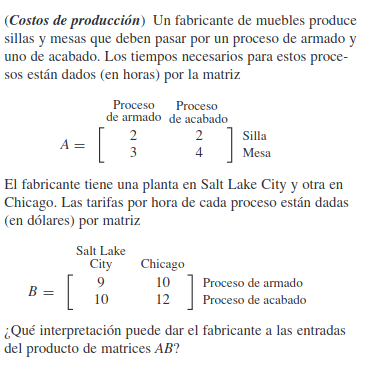
\includegraphics{figures/produccion.png}

}

\caption{Problema de Costos de Producción}

\end{figure}%

\begin{center}\rule{0.5\linewidth}{0.5pt}\end{center}

\subsubsection{Producto punto}\label{producto-punto}

Sea \(x\) un vector de tamaño \(n\) y \(y\) un vector de tamaño \(n\).
El producto punto entre \(x\) y \(y\) se define como:

\[ x \cdot y = \sum_{i=1}^n x_i y_i \]

\begin{center}\rule{0.5\linewidth}{0.5pt}\end{center}

\textbf{Aplicación} (Aplicación: cálculo de la calificación promedio de
un curso) Suponga que un profesor utiliza cuatro notas para determinar
la calificación promedio que obtiene un estudiante en un curso:
cuestionarios, dos exámenes de una hora y un examen final. Cada una de
estas notas tiene una ponderación de 10, 30, 30 y 30\%, respectivamente.
Si las calificaciones de un estudiante son, en cada rubro, 78, 84, 62 y
85, podemos calcular el promedio del curso haciendo

\[w=\begin{bmatrix}0.1 \\ 0.3 \\ 0.3 \\ 0.3\end{bmatrix},\ \ x=\begin{bmatrix}78 \\ 84 \\ 62 \\ 85\end{bmatrix}\]

\[w \cdot x = 0.1 \cdot 78 + 0.3 \cdot 84 + 0.3 \cdot 62 + 0.3 \cdot 85 = 77.1\]

\begin{center}\rule{0.5\linewidth}{0.5pt}\end{center}

\subsubsection{Definición de Matriz
Transpuesta}\label{definiciuxf3n-de-matriz-transpuesta}

La \textbf{matriz transpuesta} de una matriz \(A\), denotada como
\(A^T\), se define como la matriz obtenida al intercambiar las filas por
columnas de \(A\). Si \(A\) es una matriz de dimensiones \(m \times n\),
entonces \(A^T\) tendrá dimensiones \(n \times m\). Matemáticamente,
esto se puede escribir como:

\[
(A^T)_{ij} = A_{ji}
\]

donde \(i\) y \(j\) representan índices de filas y columnas
respectivamente.

\begin{center}\rule{0.5\linewidth}{0.5pt}\end{center}

\subsubsection{Definición de Matriz
Simétrica}\label{definiciuxf3n-de-matriz-simuxe9trica}

Una \textbf{matriz simétrica} es una matriz cuadrada \(A\) que es igual
a su transpuesta, es decir, \(A = A^T\). Esto implica que los elementos
de la matriz son simétricos respecto a su diagonal principal.
Formalmente, una matriz \(A\) es simétrica si:

\[
A_{ij} = A_{ji}
\]

para todos los índices \(i\) y \(j\). Esto significa que el elemento en
la fila \(i\) y columna \(j\) es igual al elemento en la fila \(j\) y
columna \(i\).

\begin{center}\rule{0.5\linewidth}{0.5pt}\end{center}

\subsubsection{Definición de Matriz
Identidad}\label{definiciuxf3n-de-matriz-identidad}

La \textbf{matriz identidad} \(I\), de tamaño \(n \times n\), es una
matriz cuadrada que tiene todos sus elementos iguales a 0 excepto los de
la diagonal principal, que son iguales a 1. Esto se puede expresar como:

\[
I_{ij} = 
\begin{cases} 
1 & \text{si } i = j \\
0 & \text{si } i \neq j
\end{cases}
\]

La multiplicación de matrices, es decir, para cualquier matriz \(A\) de
tamaño \(n \times n\), se cumple que:

\[
AI = IA = A
\]

\begin{center}\rule{0.5\linewidth}{0.5pt}\end{center}

\subsubsection{Definición de Matriz
Inversa}\label{definiciuxf3n-de-matriz-inversa}

La \textbf{matriz inversa} de una matriz cuadrada \(A\), denotada como
\(A^{-1}\), es aquella que, cuando se multiplica por \(A\), resulta en
la matriz identidad \(I\). Esto se expresa como:

\[
AA^{-1} = A^{-1}A = I
\]

Para que una matriz \(A\) tenga inversa, debe ser cuadrada y su
determinante no debe ser cero. La matriz inversa se utiliza para
resolver sistemas de ecuaciones lineales y en la teoría de
transformaciones lineales.

\begin{center}\rule{0.5\linewidth}{0.5pt}\end{center}

\subsubsection{Ejemplo de Matriz
Inversa}\label{ejemplo-de-matriz-inversa}

Considere la matriz \(A\):

\[
A = \begin{bmatrix}
1 & 2 \\
3 & 4
\end{bmatrix}
\]

La matriz inversa es \[
A^{-1} = \begin{bmatrix}
-2 & 1 \\
1.5 & -0.5
\end{bmatrix}
\]

\begin{center}\rule{0.5\linewidth}{0.5pt}\end{center}

\subsubsection{Combinaciones lineales}\label{combinaciones-lineales}

Una combinación lineal de un conjunto de vectores
\(\{v_1, v_2, \ldots, v_n\}\) es una expresión de la forma:

\[ c_1 v_1 + c_2 v_2 + \ldots + c_n v_n \]

Donde \(c_1, c_2, \ldots, c_n\) son escalares.

\begin{center}\rule{0.5\linewidth}{0.5pt}\end{center}

\textbf{Ejemplo de combinación lineal}

\subsubsection{Ejemplo de Combinación Lineal de Vectores de Tres
Dimensiones}\label{ejemplo-de-combinaciuxf3n-lineal-de-vectores-de-tres-dimensiones}

Consideremos los siguientes vectores en \(\mathbb{R}^3\):

\[
\mathbf{v}_1 = \begin{pmatrix}
1 \\
2 \\
3
\end{pmatrix}, \quad \mathbf{v}_2 = \begin{pmatrix}
4 \\
5 \\
6
\end{pmatrix}, \quad \mathbf{v}_3 = \begin{pmatrix}
7 \\
8 \\
9
\end{pmatrix}
\]

Una \textbf{combinación lineal} de estos vectores se forma al tomar
escalares \(\alpha, \beta, \gamma\), que pueden ser cualquier número
real, y combinar los vectores de la siguiente manera:

\[
\alpha \mathbf{v}_1 + \beta \mathbf{v}_2 + \gamma \mathbf{v}_3
\]

\begin{center}\rule{0.5\linewidth}{0.5pt}\end{center}

Por ejemplo, si elegimos \(\alpha = 1\), \(\beta = -2\), y
\(\gamma = 3\), la combinación lineal sería:

\[
1 \cdot \begin{pmatrix}
1 \\
2 \\
3
\end{pmatrix} - 2 \cdot \begin{pmatrix}
4 \\
5 \\
6
\end{pmatrix} + 3 \cdot \begin{pmatrix}
7 \\
8 \\
9
\end{pmatrix} = \begin{pmatrix}
1 \cdot 1 - 2 \cdot 4 + 3 \cdot 7 \\
1 \cdot 2 - 2 \cdot 5 + 3 \cdot 8 \\
1 \cdot 3 - 2 \cdot 6 + 3 \cdot 9
\end{pmatrix} = \begin{pmatrix}
14 \\
13 \\
12
\end{pmatrix}
\]

\begin{longtable}[]{@{}
  >{\raggedright\arraybackslash}p{(\columnwidth - 0\tabcolsep) * \real{0.0417}}@{}}
\toprule\noalign{}
\endhead
\bottomrule\noalign{}
\endlastfoot
Este resultado, \(\begin{pmatrix}
14 \\
13 \\
12
\end{pmatrix}\), es un vector en \(\mathbb{R}^3\) que es una combinación
lineal de \(\mathbf{v}_1\), \(\mathbf{v}_2\), y \(\mathbf{v}_3\) con los
coeficientes 1, -2, y 3 respectivamente. \\
\end{longtable}

\subsection{Sistema de ecuaciones
lineales}\label{sistema-de-ecuaciones-lineales}

Un \textbf{sistema de ecuaciones lineales} es un conjunto de ecuaciones
lineales que comparten las mismas variables. Un sistema de ecuaciones
lineales puede tener una o más soluciones, dependiendo de la cantidad de
ecuaciones y variables. Un sistema de ecuaciones lineales se puede
representar de la siguiente manera:

\[ a_{11} x_1 + a_{12} x_2 + \ldots + a_{1n} x_n = b_1 \]
\[ a_{21} x_1 + a_{22} x_2 + \ldots + a_{2n} x_n = b_2 \] \[ \vdots \]
\[ a_{m1} x_1 + a_{m2} x_2 + \ldots + a_{mn} x_n = b_m \] Donde:

\begin{itemize}
\tightlist
\item
  \(a_{ij}\) son los coeficientes de las variables
\item
  \(x_i\) son las variables
\item
  \(b_i\) son los términos constantes
\item
  \(m\) es el número de ecuaciones
\item
  \(n\) es el número de variables
\end{itemize}

\begin{center}\rule{0.5\linewidth}{0.5pt}\end{center}

\subsubsection{Ejemplo de Sistema de Ecuaciones
Lineales}\label{ejemplo-de-sistema-de-ecuaciones-lineales}

Considere el siguiente sistema de ecuaciones lineales:

\[ 2x + 3y = 7 \] \[ 4x - y = 7 \]

Para resolver este sistema, podemos usar el método de eliminación o
sustitución. En este caso, podemos resolver el sistema de ecuaciones
lineales para encontrar que \(x = 2\) y \(y = 1\).

\begin{center}\rule{0.5\linewidth}{0.5pt}\end{center}

Note que el vector

\[2\begin{pmatrix}2 \\
 4\end{pmatrix}+1\begin{pmatrix}3\\-1\end{pmatrix}=\begin{pmatrix}7\\7\end{pmatrix}\]

¿Qué significa esto? ¿Como podemos encontrar la solcuión de un sistema
de ecuaciones lineales?

\begin{center}\rule{0.5\linewidth}{0.5pt}\end{center}

\subsection{Ejemplo 2}\label{ejemplo-2}

veamos otro ejemplo

\[ 3x + 2y = 11 \] \[ 2x - y = 5 \] \[ 5x + 3y = 18 \]

Note que el vector

\[2\begin{pmatrix}3 \\ 2\\ 5
 \end{pmatrix}+1\begin{pmatrix}2\\-1\\ 3\end{pmatrix}=\begin{pmatrix}11\\5\\18\end{pmatrix}\]

\begin{center}\rule{0.5\linewidth}{0.5pt}\end{center}

Note que podemos encontrar la solución de un sistema de ecuaciones
lineales como una combinación lineal de los vectores que representan las
ecuaciones.

Podemos estudiar sistemas de diferentes dimensiones. Aunque, en primera
parte de este curso nos enfocaremos en sistemas cuadrados. es decir, que
tengan el mismo numero de filas y columnas.

\begin{center}\rule{0.5\linewidth}{0.5pt}\end{center}

\subsubsection{Solución de un Sistema de Ecuaciones
Lineales}\label{soluciuxf3n-de-un-sistema-de-ecuaciones-lineales}

\begin{itemize}
\tightlist
\item
  Sustitución
\item
  Eliminación
\item
  Reducción
\end{itemize}

\begin{center}\rule{0.5\linewidth}{0.5pt}\end{center}

\subsubsection{solución de un sistema de ecuaciones lineales
triangular}\label{soluciuxf3n-de-un-sistema-de-ecuaciones-lineales-triangular}

Ejemplo:

\[  3x + 2y + z = 1 \] \[  0x - 2y + 2z = 2 \] \[  0x + 0y + 5z = 5 \]

Para resolver este sistema encontramos la solución de la tercera
ecuación y sustituimos en la segunda ecuación y luego en la primera
ecuación.

\begin{center}\rule{0.5\linewidth}{0.5pt}\end{center}

\subsubsection{Ejercicio}\label{ejercicio}

Resuelva el siguiente sistema de ecuaciones lineales:

\[ 2x + 3y +z -w= 7 \] \[ 0x - 2y + 2z +w = 2 \]
\[ 0x + 0y + 5z -w = 5 \] \[ 0x + 0y + 0z +w = 1 \]

\begin{center}\rule{0.5\linewidth}{0.5pt}\end{center}

\subsubsection{Operaciones elementales de
matrices}\label{operaciones-elementales-de-matrices}

Las operaciones elementales de matrices son operaciones que se pueden
realizar en las filas de una matriz sin cambiar la solución de un
sistema de ecuaciones lineales. Estas operaciones incluyen:

\begin{itemize}
\tightlist
\item
  Intercambiar dos filas
\item
  Multiplicar una fila por un escalar no nulo
\item
  Sumar un múltiplo de una fila a otra fila
\end{itemize}

Estas operaciones se utilizan para simplificar una matriz y facilitar la
resolución de un sistema de ecuaciones lineales.

\begin{center}\rule{0.5\linewidth}{0.5pt}\end{center}

\subsubsection{Ejemplo de Operaciones Elementales de
Matrices}\label{ejemplo-de-operaciones-elementales-de-matrices}

Considere la siguiente matriz:

\$\$

\begin{bmatrix}

1 & 2 & 3 \\

4 & 5 & 6 \\

7 & 8 & 9

\end{bmatrix}

\begin{center}\rule{0.5\linewidth}{0.5pt}\end{center}

¿Cómo podemos usar las operaciones elementales para solucionar un
sistema de ecuaciones lineales?




\end{document}
